% Figure 2: retain the reviewed PNG artwork and typeset legible vector labels.
% The source PNG is unchanged. Labels are 8.6 pt Times New Roman before the
% report's small reduction. The art and model content are retained; duplicated
% footer notes are omitted because the caption/body already explain them.
% Rebuild with: python final_report/prepare_report.py --overview-only
\documentclass[border=0pt]{standalone}
\usepackage{graphicx}
\usepackage{fontspec}
\setmainfont{Times New Roman}
\usepackage{tikz}
\definecolor{normalfill}{HTML}{D4E5F7}
\definecolor{stalefill}{HTML}{DAF2E8}
\definecolor{headfill}{HTML}{C4EDDF}
\definecolor{meanfill}{HTML}{FFF0C7}
\definecolor{barfill}{HTML}{64D5BD}
\begin{document}
\begin{tikzpicture}[x=.2320442bp,y=-.2320442bp,
  every node/.style={font=\fontsize{8.6}{9.6}\selectfont,
                    align=center,inner sep=0pt,outer sep=0pt}]
\useasboundingbox (0,0) rectangle (2172,630);
\begin{scope}
\clip (0,0) rectangle (2172,630);
\node[anchor=north west] at (0,0) {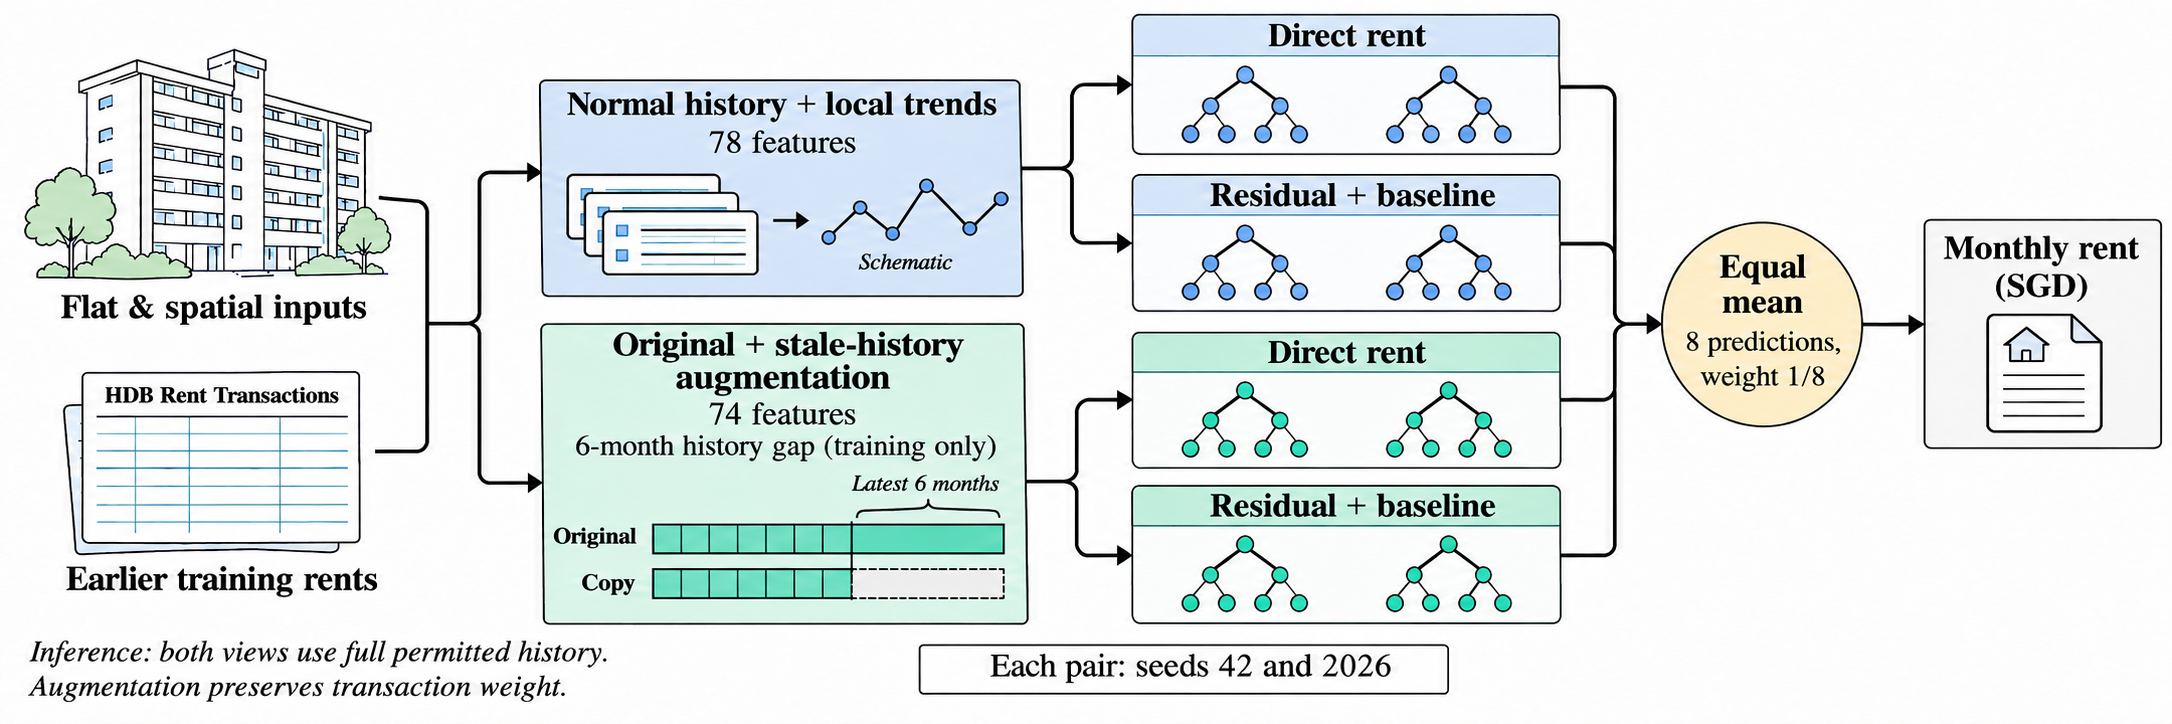
\includegraphics[width=7in]{model_overview.png}};
% Retype labels, not the artwork, at a consistent publication-size font.
\fill[white] (20,283) rectangle (400,333);
\node[font=\fontsize{8.6}{9.6}\selectfont\bfseries] at (210,307) {Flat \& spatial inputs};
\fill[white] (85,377) rectangle (356,415);
\node[font=\fontsize{8.6}{9.6}\selectfont\bfseries] at (221,396) {HDB rents};
\fill[white] (50,557) rectangle (410,609);
\node[font=\fontsize{8.6}{9.6}\selectfont\bfseries] at (225,582) {Earlier training rents};

\fill[normalfill] (545,84) rectangle (1015,164);
\node[font=\fontsize{8.6}{9.6}\selectfont\bfseries] at (780,107) {Normal history + local trends};
\node at (780,146) {78 features};
\fill[normalfill] (838,242) rectangle (984,282);
\node[font=\fontsize{8.6}{9.6}\selectfont\itshape] at (907,263) {Schematic};

\fill[stalefill] (547,329) rectangle (1018,470);
\node[font=\fontsize{8.6}{9.6}\selectfont\bfseries] at (783,350) {Original + stale-history};
\node at (783,391) {augmentation: 74 features};
\node at (783,440) {6-month gap (training only)};
\fill[stalefill] (766,472) rectangle (1017,499);
\node[anchor=east,font=\fontsize{8.6}{9.6}\selectfont\itshape] at (1003,484) {Latest 6 months};
% Re-space the two illustrative strips so their row labels fit at 8+ pt.
\fill[stalefill] (548,520) rectangle (1017,607);
\node[anchor=east] at (674,539) {Original};
\node[anchor=east] at (674,584) {Copy};
\filldraw[fill=barfill,draw=black,line width=.4pt] (688,525) rectangle (1004,553);
\filldraw[fill=barfill,draw=black,line width=.4pt] (688,570) rectangle (852,598);
\filldraw[fill=white,draw=black,dashed,line width=.4pt] (852,570) rectangle (1004,598);
\foreach \xx in {708.5,729,749.5,770,790.5,811,831.5,852} {
  \draw[line width=.3pt] (\xx,525) -- (\xx,553);
  \draw[line width=.3pt] (\xx,570) -- (\xx,598);
}

\foreach \top/\bottom/\mid/\tone/\heading in {
  18/53/35/normalfill/Direct rent,
  179/213/195/normalfill/Residual + baseline,
  337/370/353/headfill/Direct rent,
  490/524/507/headfill/Residual + baseline} {
  \fill[\tone] (1137,\top) rectangle (1553,\bottom);
  \node[font=\fontsize{8.6}{9.6}\selectfont\bfseries] at (1345,\mid) {\heading};
}
\fill[meanfill] (1762,324) circle (97);
\node[font=\fontsize{8.6}{9.6}\selectfont\bfseries] at (1762,269) {Equal};
\node[font=\fontsize{8.6}{9.6}\selectfont\bfseries] at (1762,306) {mean};
\node at (1762,346) {8 outputs};
\node at (1762,382) {weight 1/8};
\fill[white] (1930,225) rectangle (2155,304);
\node[font=\fontsize{8.6}{9.6}\selectfont\bfseries] at (2042,247) {Monthly rent};
\node at (2042,286) {(SGD)};

\end{scope}
\end{tikzpicture}%
\end{document}
